%\section{Evolutionary Algorithm-based Optimization}
\section{Comparative Evolutionary Optimization}
\label{sec:optimization}
Once the CHP plant has been modeled by means of the connected NNs, the next step is to  carry out an optimization process to improve the efficiency of the whole process. In particular, we focus on three performance objectives: 1) minimizing the amount of used fuel $Q_{fuel}$ (i.e., natural gas flow); 2) maximizing the useful thermal energy $FE_v$ (i.e., flow of the fluent in the evaporator) and 3) maximizing the generated power $POW$. Therefore, we have actually a multi-objective optimization problem. To perform this process, a total of twelve decision variables  are available in the plant; that is, a set of input variables whose values can be changed freely (within certain bounds) by the user. These twelve variables are those highlighted in bold in Table \ref{fignns}. The mathematical formulation of this multi-objective problem is as follows:
%
\begin{itemize}[-]
	\item Minimize used fuel: $Q_{fuel} = F_{Gas_A} + F_{Gas_B} + F_{Gas_C} + F_{Gas_D}$.
	\item Maximize drying process: $F_{Ev}$.
	\item Maximize power: $POW = POW_A + POW_B + POW_C + POW_D + POW_{ST}$.
\end{itemize}
%
The decision variables and their restrictions are listed below:
%
\begin{itemize}[-]
	\item $T_{B1\_A}, T_{B2\_A}, T_{B1\_B}, T_{B2\_B}, T_{B1\_C}, T_{B2\_C}, T_{B1\_D}, T_{B1\_D}$. (i.e., two air intake temperatures for each engine): $\SI{30}{\celsius} \leq T  \leq  \SI{38}{\celsius}$.
	\item $T_{H2O\_Ex}$ (exchange water temperature): $\SI{61}{\celsius}  \leq T  \leq  \SI{65}{\celsius}$.
	\item $P_{St\_Gen}$ (pressure of the steam generator): $\SI{20}{bar}  \leq  P  \leq  \SI{22}{bar}$.
	\item $P_{Ev}$ (evaporator pressure): $\SI{0.13}{bar}  \leq  P  \leq  \SI{0.17}{bar}$.
	\item $T_{H2O\_SH}$ (superheated water temperature): $\SI{110}{\celsius}  \leq  T  \leq  \SI{125}{\celsius}$.
\end{itemize}

Our combined approach of using NNs as black box functions may be applied in conjunction with any optimization algorithm that is able to handle real-valued decision variables. For this reason, several state-of-the-art, multiobjective evolutionary algorithms, which use different search strategies, are considered for solving the proposed optimization problem.

The difficulty in solving a multiobjective optimization problem is that there usually exists no single solution that optimizes all goals at the same time \cite{basicDeb,basicCoello}. Instead, metaheuristics aim at finding a representative approximation to the so-called Pareto optimal front. The Pareto front comprises all solutions that can only be improved in one objective by impairing at least one other objective. The idea is that a decision maker chooses a solution to implement from this approximation. The approximation of a Pareto front is graded with respect to two criteria. The points found by an algorithm should be located as close as possible to the Pareto front. At the same time, the approximation should cover the Pareto front in its entirety so the decision maker has full knowledge about the available options. The former aspect is denoted by convergence and the latter by diversity.

AbYSS \cite{abyss} uses a scatter search template as local search operator. ESPEA's \cite{espea} niching technique is inspired by the physical phenomenon of electrostatic potential energy. Indicator-based selection guides the search mechanism of IBEA \cite{ibea}. MOEA/D \cite{moead2009} simultaneously solves multiple scalarized instances of the original problem. NSGA-II \cite{nsga2} uses a domination based topological sorting and the crowding distance metric as niching technique. It's successor, NSGA-III \cite{nsga3part1}, applies a reference point based search method. SMS-EMOA \cite{smsemoa} aims at finding a population that maximizes the so-called hypervolume measure. Finally, SMPSO \cite{smpso} is a particle swarm optimization approach. We have performed an extensive computational study making use of the jMetal framework version 4.5 \cite{jmetal2}, in order to assess the performance of these individual algorithms. Our code and resources are hosted online on Sourceforge and are publicly available\footnote{\url{http://sourceforge.net/projects/jmetalbymarlonso/}}.

As stated before, the performance of the CHP plant is influenced by 213 different parameters of which 36 were found to have a significant impact as indicated in Table \ref{fignns}. While twelve of these parameters may be manipulated by the plant operator as decision variables, there still exist 24 parameters, whose different combinations of values potentially affect the optimization effort.
%
We therefore randomly picked 39 parameter observations from our database, which come from a week of the month February and serve as representative sample. For each observation, we extracted the values of those 24 parameters that affect the plant operation and cannot be manipulated by the operator. These 24 parameters of each of the 39 observations serve as individual problem instances for our computational study. 
%
%Therefore, we picked a representative sample of 39 parameter combinations from the month February from our data base that serve as different problem instances for a computational study.
The objective of this study is identifying the algorithm that delivers the best performance by choosing optimal values for the twelve decision variables across all 39 problem instances. Each algorithm was run 100 times on every problem instance employing a population size of 100. Algorithm configurations were taken from their original publications. \num{50000} function evaluations were performed per run. Preliminary tests have revealed that the populations of the algorithms assessed in this study become evolutionary stable at \num{50000} evaluations.

We chose the Inverted Generational Distance (IGD) as performance metric, since it captures both convergence and diversity \cite{van1998evolutionary}. The IGD metric computes the average of the minimum distances of every Pareto optimal point to a given Pareto front approximation. Since the Pareto fronts are not known in our case, we use all nondominated solutions obtained across all algorithm runs of a single problem instance as reference front (an example is given in Figure \ref{fig:paretofront}). Objective values were normalized to mitigate the effect of different scales.

A preliminary analysis has revealed that the performance of an individual algorithm only differs marginally across the different problem instances. This observation indicates that our approach is very robust with respect to the parameters that cannot be influenced by the operator. For the sake of clarity, we therefore only provide a summary of the results in Table \ref{tbl:summary}. Full results are provided in the appendix in Table \ref{table:median.IGD}.

\begin{table}
\caption{Mean and standard deviation (as subscript) of median IGD across all test problems.}
\label{tbl:summary}
\centering
\begin{tabular}{*{4}{c}} \toprule
AbYSS & ESPEA & IBEA & MOEAD\\ \cmidrule(lr){1-1} \cmidrule(lr){2-2} \cmidrule(lr){3-3} \cmidrule(lr){4-4}
$\num{3.41E-4}_{\num{2.13E-5}}$ & $\num{1.69e-4}_{\num{1.92e-5}}$ & $\num{1.53E-3}_{\num{1.88E-4}}$ & $\num{1.51E-3}_{\num{1.72E-4}}$ \\ \midrule
NSGA-II & NSGA-III & SMPSO & SMS-EMOA \\ \cmidrule(lr){1-1} \cmidrule(lr){2-2} \cmidrule(lr){3-3} \cmidrule(lr){4-4}
$\num{3.55E-4}_{\num{2.20E-5}}$ & $\num{1.25E-3}_{\num{1.33E-4}}$ & $\num{3.30E-4}_{\num{2.07E-5}}$ & $\num{1.53E-3}_{\num{1.68E-4}}$ \\
\bottomrule
\end{tabular}
\end{table}

The study results demonstrate that there exist clear performance differences between individual algorithms. Values of the IGD metric differ by a factor of ten from best to worst. This implies that the choice of algorithm greatly influences the optimization outcome. Best results are obtained using ESPEA, whereas AbYSS, NSGA-II and SMPSO show also good performances. IBEA, MOEA/D, NSGA-III and SMS-EMOA, on the other hand, trail behind. The smallest average IGD is achieved by ESPEA. A Kruskal-Wallis test \cite{kruskal1952use} in conjunction with a post-hoc analysis has revealed that the difference in IGD values between ESPEA and the other algorithms across all 39 problems is significant.\footnote{P-values were equal to zero in our analysis.}

\begin{figure}
\centering
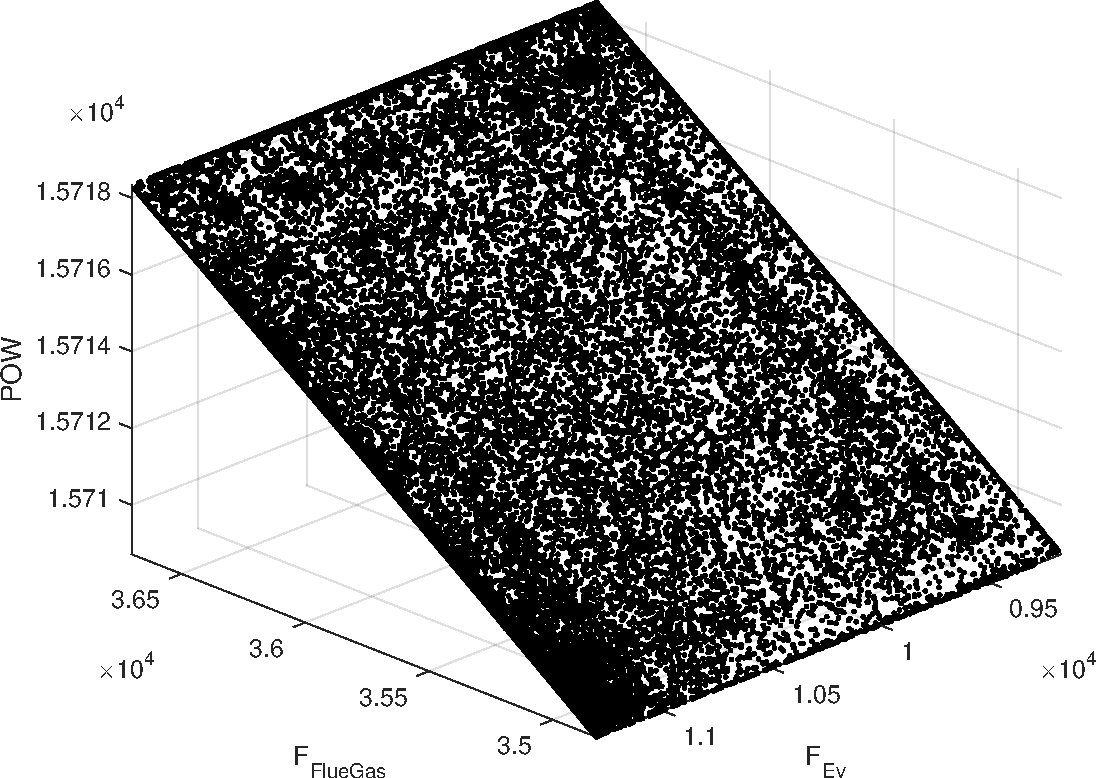
\includegraphics[width=0.7\textwidth]{figures/paretofront_cropped.pdf}
\caption{Pareto front of problem instance 2 out of 39 of the cogeneration optimization problem. The front is a collection of all non-dominated solutions that were retrieved in final populations during the study.}
\label{fig:paretofront}
\end{figure}

A closer analysis of the Pareto front reveals possible explanations for the performance differences observed. Figure \ref{fig:paretofront} shows the Pareto front of a cogeneration optimization problem instance. The rectangular shape of the front suggests that all Pareto optimal points lie on a plane. A regression analysis has indeed confirmed that, for 38 out of 39 problem instances, all points can be fitted in a plane with a coefficient of determination of 1.\footnote{The Pareto front of problem instance 1 out 39 (referenced as CG0 in Table \ref{table:median.IGD}) consists of two different planes.} Strikingly, the Pareto front is linear, whereas the problem itself is not.

\begin{figure}
\centering
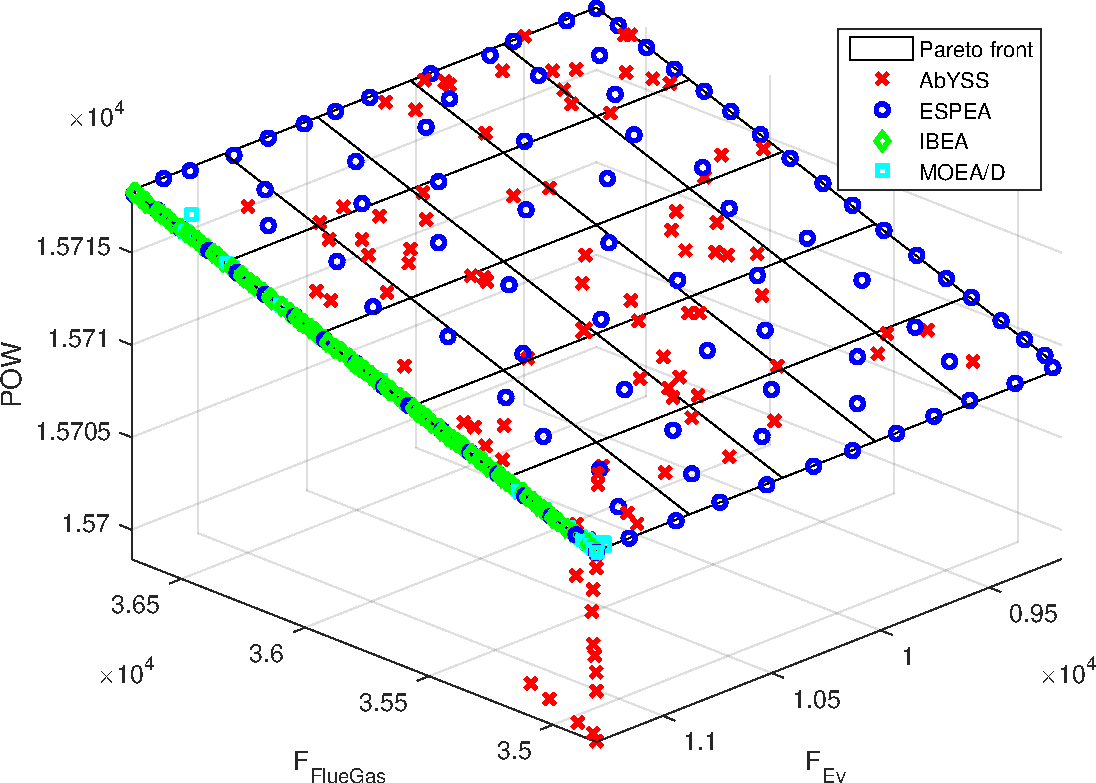
\includegraphics[width=0.7\textwidth]{figures/example1_cropped.pdf}
\caption{Exemplary search results of the algorithms AbYSS, ESPEA, IBEA and MOEA/D on problem instance 2 for illustrating their performance.}
\label{fig:exruns1}
\end{figure}

Figures \ref{fig:exruns1} and \ref{fig:exruns2} offer an explanation to why algorithm performances can be divided into two tiers. AbYSS, ESPEA, NSGA-II and SMPSO capture the extent of the Pareto front in its entirety, whereas ESPEA achieves the most equidistant approximation. NSGA-II and AbYSS retrieve several dominated points as indicated in the plot. IBEA, MOEA/D, NSGA-III and SMS-EMOA focus mainly on a single edge of the front. We believe that using reference points from \cite{nbi} as it is suggested in \cite{moead2009,nsga3part1} is problematic given the presented front. We assume that the reference points do not cover the front equally, which leads to a strong focus on boundary solutions. A better choice of reference points might ameliorate this issue. Hypervolume-based methods, such as SMS-EMOA and the IBEA configuration used in this study, seem to struggle with the geometry of the front. We speculate that, despite objective normalization, boundary points yield the highest hypervolume contributions on plane-shaped fronts. Although the figures only depict single runs, these basic observations could be confirmed for other problem instances and different runs as well.

\begin{figure}
\centering
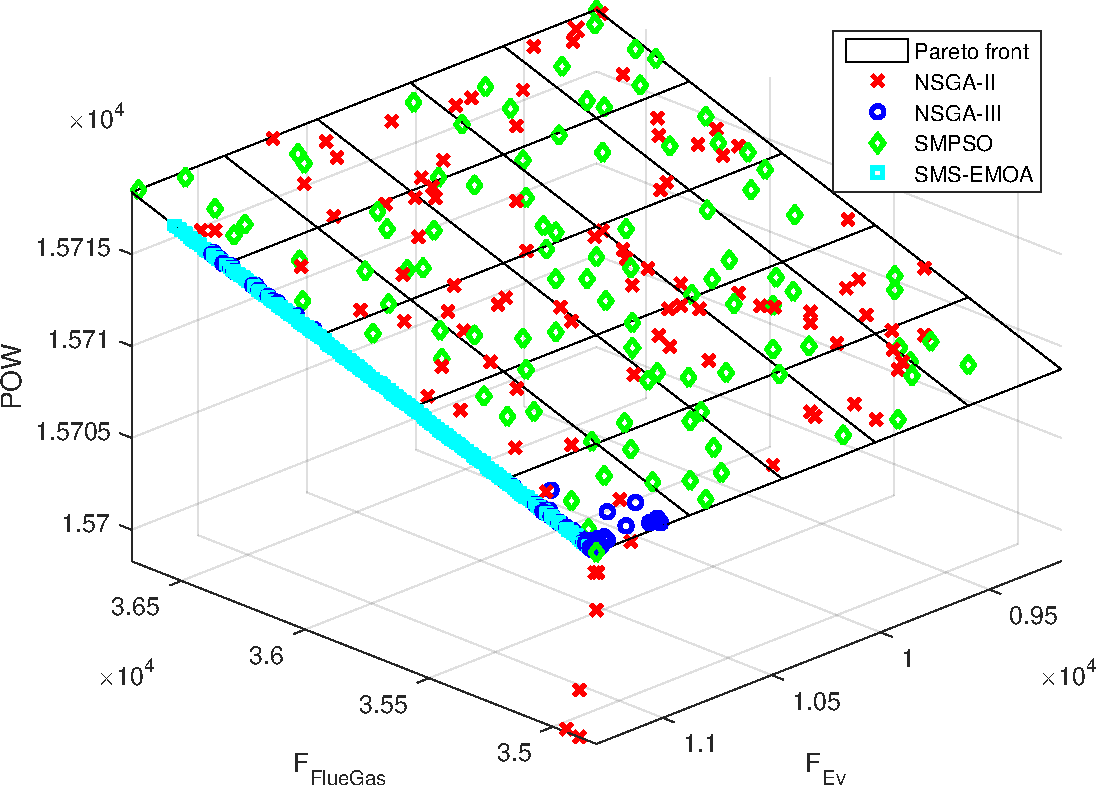
\includegraphics[width=0.7\textwidth]{figures/example2_cropped.pdf}
\caption{Exemplary search results of the algorithms NSGA-II, NSGA-III, SMPSO and SMS-EMOA on problem instance 2 for illustrating their performance.}
\label{fig:exruns2}
\end{figure}

Robustness is another aspect of algorithm performance that is of interest in our setting. In practice, it is usually not feasible to conduct 100 runs and choose the most preferable option from this pool of alternatives. If there is little variability between the results of individual runs, however, we can conclude that every single run yields a satisfying approximation of the Pareto front. One way of assessing robustness is considering the surface attainment \cite{fonseca1996performance} across multiple runs. Surface attainment measures the space that is dominated by a given approximation set. When measured across multiple runs, surface attainment yields the space that is dominated in a given percentage of runs. Figure \ref{fig:surfaceattainment} provides an example for the visualization of the surface attainment of ESPEA of the first and 100th percentile. We can see that both surfaces nearly coincide, further indicating that our optimization approach is very robust across different runs. Similar observations were made for other problem instances.

\begin{figure}
	\begin{subfigure}{0.47\textwidth}
	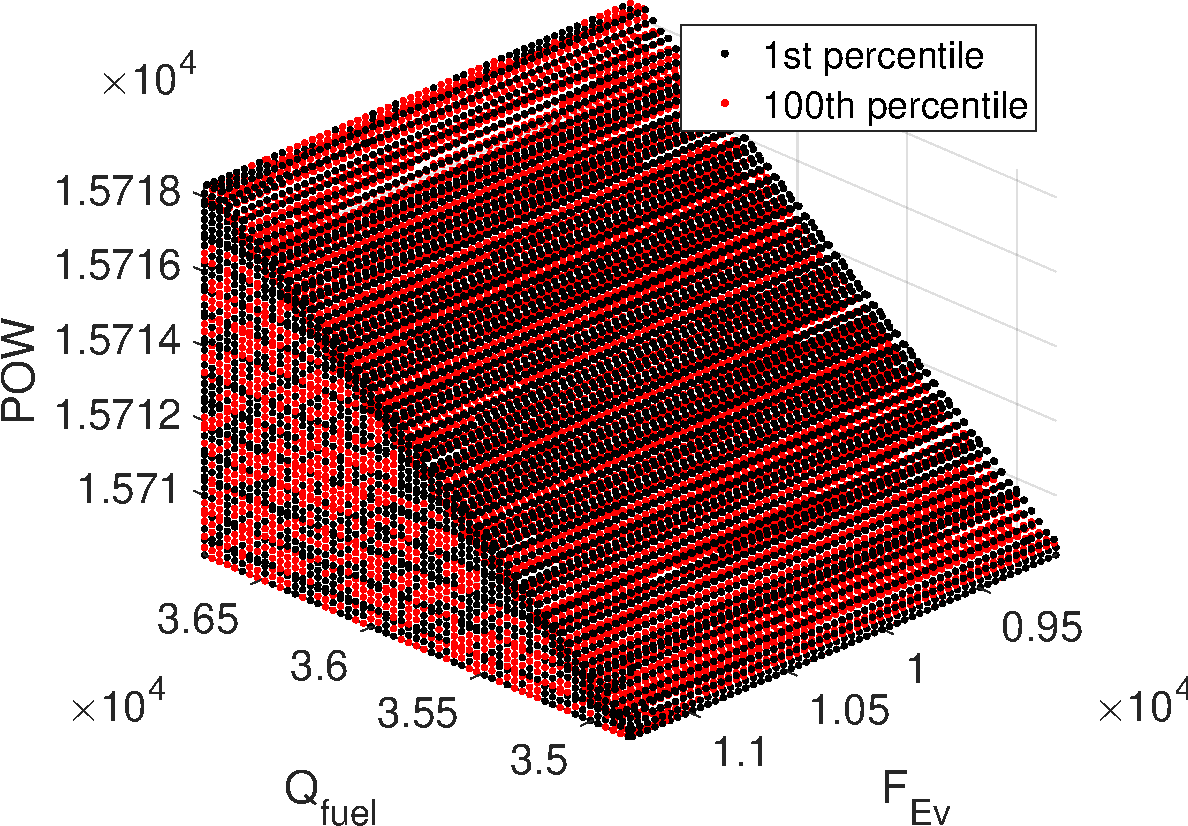
\includegraphics[width=\textwidth]{figures/safront_cropped.pdf}
	\end{subfigure}
\hfill
	\begin{subfigure}{0.47\textwidth}
	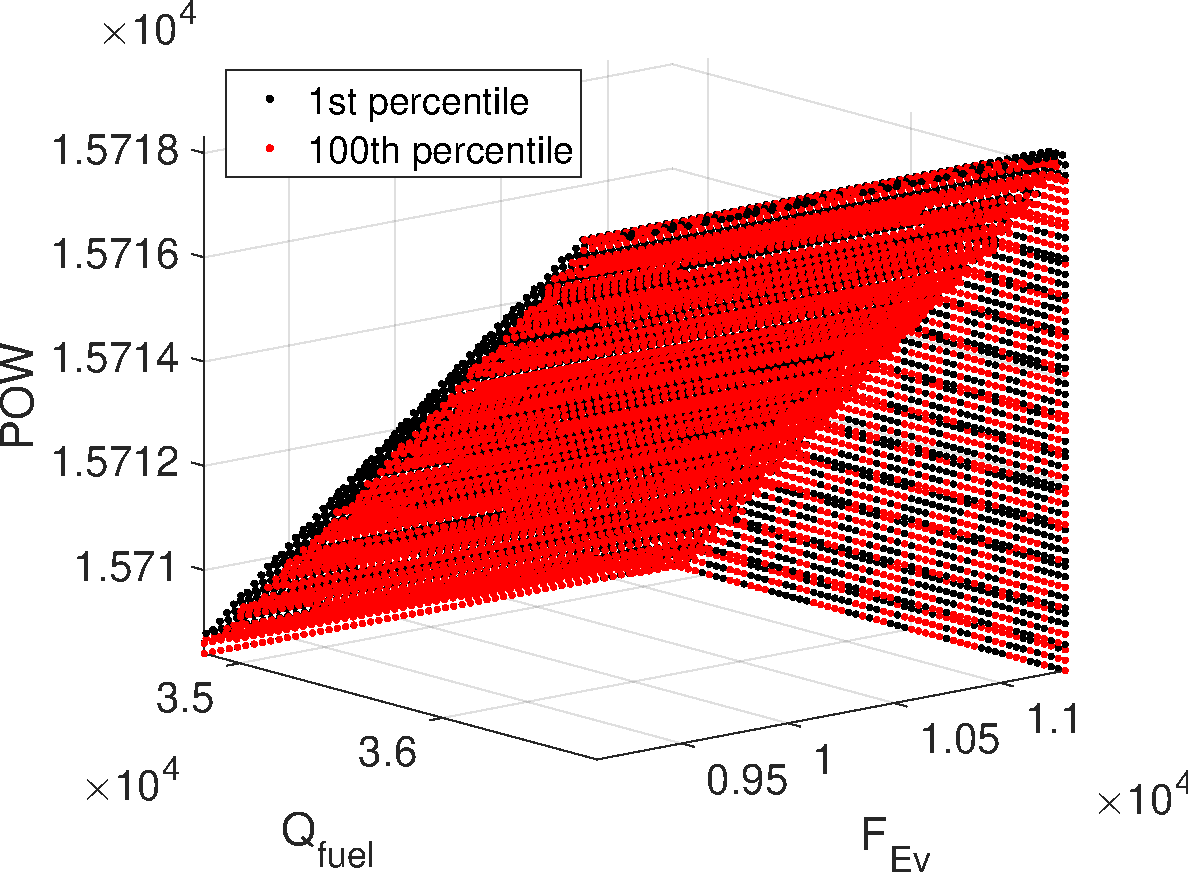
\includegraphics[width=\textwidth]{figures/saback_cropped.pdf}
	\end{subfigure}
\caption{Surface attainment plot of ESPEA for the first and 100th percentile of problem instance 2 from the front (left) and the back (right). The first percentile depicts the space that is dominated by all ESPEA runs combined, while the 100th percentile shows the space that is dominated in all of the 100 runs.}
\label{fig:surfaceattainment}
\end{figure}

The multiobjective approach generates a set of solutions among which a decision maker chooses an option that fits his preferences best. In the present context, there exists an efficiency measure that may be used to evaluate the quality of the cogeneration process. Efficiency can be defined as a quotient of the power generated by the unused energy contained in the fuel:
%
\begin{equation}
\label{eq:efficiency}
\varepsilon_{EE} = \frac{100 \cdot POW}{Q_{fuel} - F_{Ev}/0.9}.
\end{equation}
%
A question that needs to be addressed in this context is, whether the multi-objective approach is suited to find a solution that maximizes the efficiency of the cogeneration process. Our computational study has revealed that all algorithms with the exception of NSGA-II and NSGA-III were able to find a solution possessing an efficiency of 70.6 on every problem instance in their median runs. The best solutions obtained by NSGA-II and NSGA-III across all problems exhibit an efficiency of 70.5. %Both values are higher than any efficiencies achieved by previous optimization efforts, where values varied largely between 61 and 70 \cite[Fig. 11]{Seijo2016309}.

If a choice rule such as (\ref{eq:efficiency}) is given, it makes sense to focus the search from the beginning on those regions of the Pareto front that yield the highest efficiency. In a multi-objective context, however, a decision maker is usually not only interest in obtaining a preconceived optimum, but also in comparing his choice to other options available \cite{roy1996multicriteria,kahneman1979prospect}.

ESPEA provides a mechanism that bridges the gap between those conflicting goals. The basic notion of this algorithm consists of interpreting the Pareto front as closed physical system in which charged particles, represented by solutions, may move freely. The aim of ESPEA is to obtain an approximation of a fixed, given size of the Pareto front that minimizes the energy of the system. For this purpose, the algorithm maintains an archive of nondominated solutions. The energy of the archive is computed as the sum of all pair-wise energies between individual solutions of the archive. In physics, the electrostatic energy that works between two particles is the product of their charges divided by their Euclidean distance. ESPEA uses the distance in objective space for computing energies. Charges are interpreted as utility values, where a lower utility corresponds to a higher desirability. In case all solutions are equally desirable, charges are set to one, as it was done for the computational study. In the second part of our analysis, we use (\ref{eq:efficiency}) as charges for biasing the search towards the efficiency optimum. Efficiency values were raised by three to increase the bias of the search as hinted at in \cite{espea}.

\begin{figure}
\centering
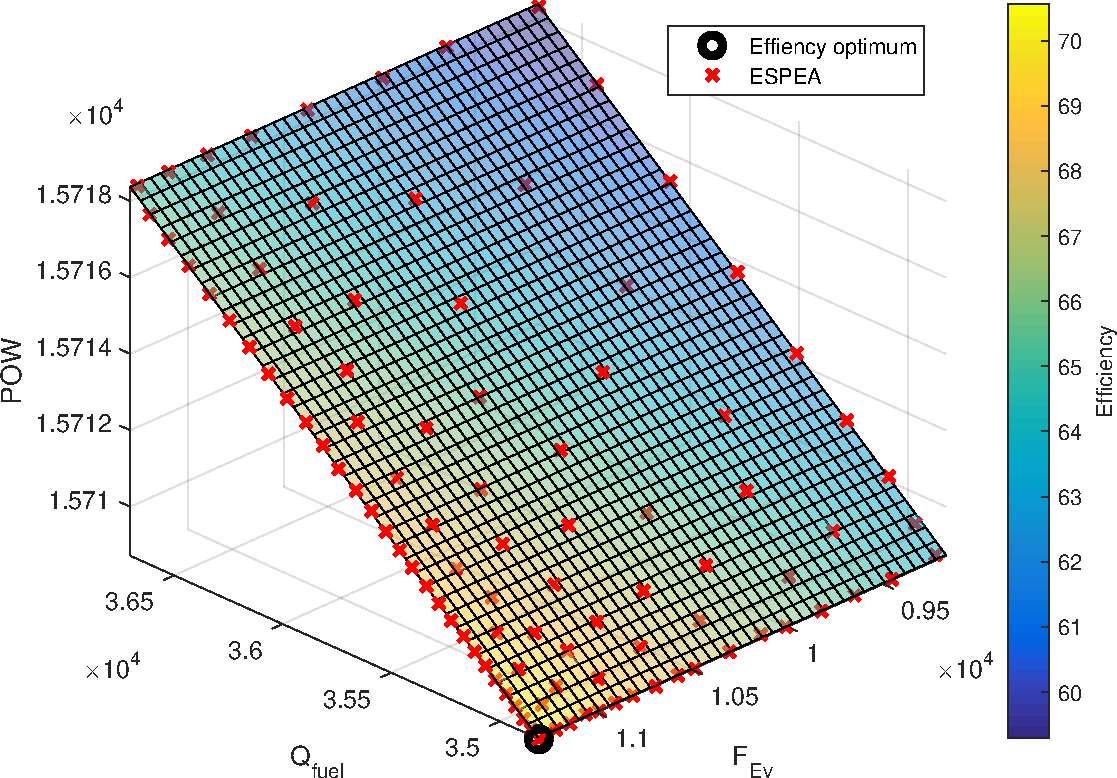
\includegraphics[width=0.7\textwidth]{figures/espeacharge_cropped.pdf}
\caption{A single run of ESPEA using efficiency values as charges on problem instance 31.}
\label{fig:espea}
\end{figure}

Figure \ref{fig:espea} illustrates the effect of using the charge mechanism in ESPEA. We observe that the density of solutions is higher in those regions that show high efficiencies. At the same time, an approximation to the Pareto front in its entirety is retained enabling the decision maker to compare the highest efficiency option to other alternatives available.

\begin{figure}
\centering
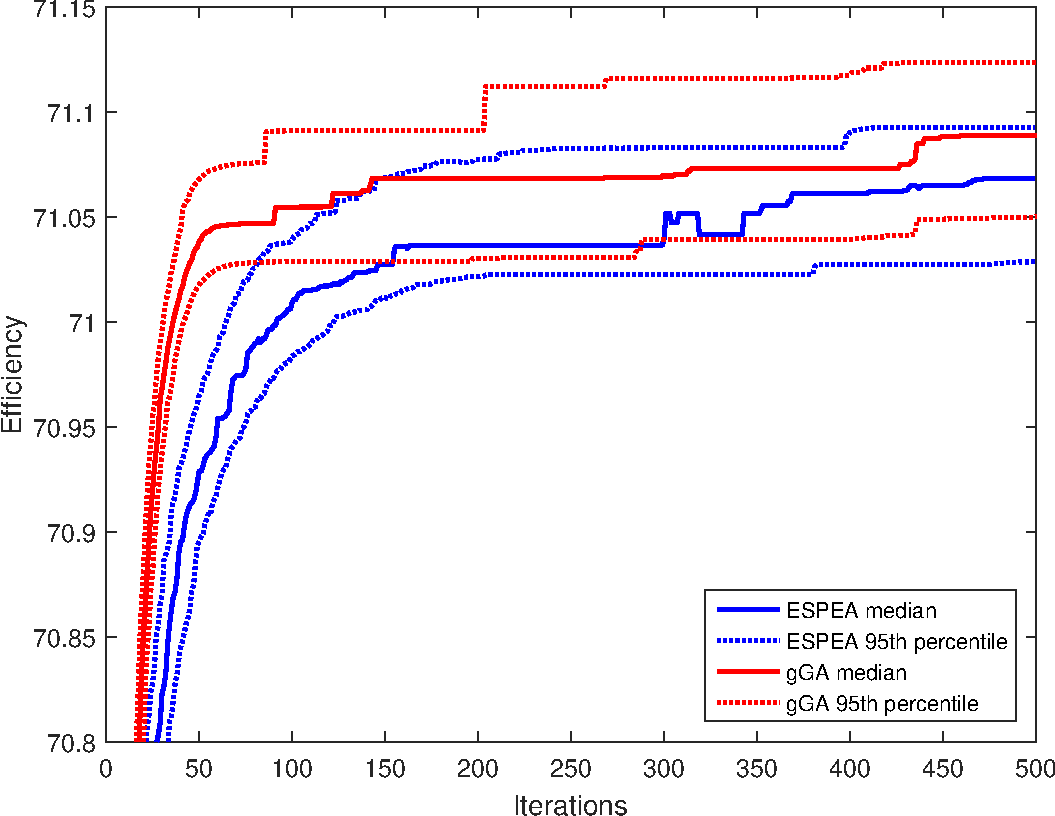
\includegraphics[width=0.7\textwidth]{figures/efficiency_cropped.pdf}
\caption{Comparison of ESPEA using efficiency values as charges to an EGGA. We computed the median and the 95th percentile of the best efficiency observed in each iteration and for every problem across all 100 runs for each algorithm. The median of medians and the 95th percentile of 95th percentiles across all 39 problems are depicted in the figure.}
\label{fig:efficiency}
\end{figure}

Using ESPEA's charge mechanism focuses the search on generating more solutions that are close to the efficiency optimum. In this context, it appears reasonable to compare ESPEA to a single-objective optimization algorithm with respect to the efficiency optima that both algorithms obtain. We have chosen an elitist generational genetic algorithm (EGGA) for this task, which uses binary tournament selection \cite{goldberg1991comparative}, simulated binary crossover \cite{sbx}, polynomial mutation \cite{polynomialmutation} and a population size of 100. The genetic operators were configured in the same way as employed by ESPEA. Figure \ref{fig:efficiency} depicts a comparison of both algorithms' performances across all test problems. Although the EGGA converges faster, especially within the first 150 iterations, the performances of both algorithms align the more function evaluations are performed. Considering absolute values, the performance differences are almost negligible.

Since the cogeneration optimization problem as presented in this work is embedded in a real-time application, algorithm run times are a critical issue in this context.
%
As mentioned before, the thermodynamical processes inside the CHP change rather slowly. Therefore, the plant is expected to be reconfigured in regular intervals of 15 minutes. After 15 minutes have elapsed, optimization is performed using the values of the 24 significant parameters that are currently observed.
%
A single algorithm run should therefore take considerably less than 15 minutes on commercial off-the-shelf medium-class computer hardware. With the exception of ESPEA and SMS-EMOA, all algorithms finish \num{50000} function evaluations within less than ten seconds on an Intel Core i5-4300U processor running Windows 8.1. A single ESPEA run takes about half a minute, whereas an SMS-EMOA execution can take up to ten minutes. Although run-times also highly depend on the implementation and the chosen programming language, the most important factor is the computational complexity of executing a single iteration of a given optimization algorithm. ESPEA and SMS-EMOA are steady-state algorithms implying that more costly operations are performed per function evaluation. SMS-EMOA, for example, computes hypervolume contributions for every member of the last non-dominated front in each iteration. Computing hypervolume contributions is an NP-hard problem \cite{hypervolumecontribution}, which consequently results in a very high run-time. Considering all this, we may draw the conclusion that every algorithm assessed in this study is suitable for an on-line implementation with the exception of SMS-EMOA.

%____________________________________
